\documentclass[a4paper,11pt]{book}
\usepackage[left=2cm,right=2cm]{geometry}

\usepackage{graphicx}
\usepackage{indentfirst}
\usepackage{hyperref}
\usepackage{listings}
\usepackage{color}
\usepackage{amsmath}


\renewcommand{\thesection}{\arabic{chapter}.\arabic{section}.}
\renewcommand{\thesubsection}{\thesection\arabic{subsection}.}


% add code customizations
\definecolor{lightgrey}{gray}{0.95}
\definecolor{eblue}{rgb}{0,0,.5}
\definecolor{ered}{rgb}{0.5,0,0}
\definecolor{egreen}{rgb}{0,0.5,0}
\lstset{%
language = Python,
%numbers = left,
frame = single,
framexleftmargin = 0pt,
framexrightmargin = 0pt,
backgroundcolor=\color{lightgrey},
keywordstyle = \color{ered},
commentstyle = \color{egreen},
stringstyle = \color{eblue},
showstringspaces=false
}


\begin{document}
\pagestyle{plain}

\chapter{Thresholding }

Hi friends,\\

This article is about \href{http://en.wikipedia.org/wiki/Thresholding_(image_processing)}{image thresholding} and its different functionalities available in OpenCV. Thresholding converts a grayscale image to a binary image (most of the time). It is highly useful for image segmentation, creating markers, masks etc.

\section{Simple Thresholding}

Here, the matter is straight forward. If pixel value is greater than a arbitrary value, it is assigned one value (may be white), else it is assigned another value (may be white).

The function used is \href{http://docs.opencv.org/modules/imgproc/doc/miscellaneous_transformations.html#cv2.threshold}{threshold()}. First param is the source image, which \textbf{should be a grayscale image}. Second param is the threshold value which is used to classify the pixel values. Third param is the maxVal which represents the value to be given if pixel value is more than (sometimes less than) the threshold value. OpenCV provides different styles of thresholding and it decided by the fourth parameter of the function. Different types are:

\begin{enumerate}
    \item cv2.THRESH\_BINARY
	\item cv2.THRESH\_BINARY\_INV
	\item cv2.THRESH\_TRUNC
	\item cv2.THRESH\_TOZERO
	\item cv2.THRESH\_TOZERO\_INV
\end{enumerate}

Two outputs are obtained. First one is a retval which I will explain later. Second output is our thresholded image.\\
 
\bigskip
\begin{lstlisting}
import cv2
import numpy as np
from matplotlib import pyplot as plt

img = cv2.imread('messi2.jpg',0)
ret,thresh1 = cv2.threshold(img,127,255,cv2.THRESH_BINARY)
ret,thresh2 = cv2.threshold(img,127,255,cv2.THRESH_BINARY_INV)
ret,thresh3 = cv2.threshold(img,127,255,cv2.THRESH_TRUNC)
ret,thresh4 = cv2.threshold(img,127,255,cv2.THRESH_TOZERO)
ret,thresh5 = cv2.threshold(img,127,255,cv2.THRESH_TOZERO_INV)

thresh = ['img','thresh1','thresh2','thresh3','thresh4','thresh5']

for i in xrange(6):
    plt.subplot(2,3,i+1),plt.imshow(eval(thresh[i]),'gray')
    plt.title(thresh[i])

plt.show()
\end{lstlisting}
\bigskip


\begin{figure}[htp]
\centering
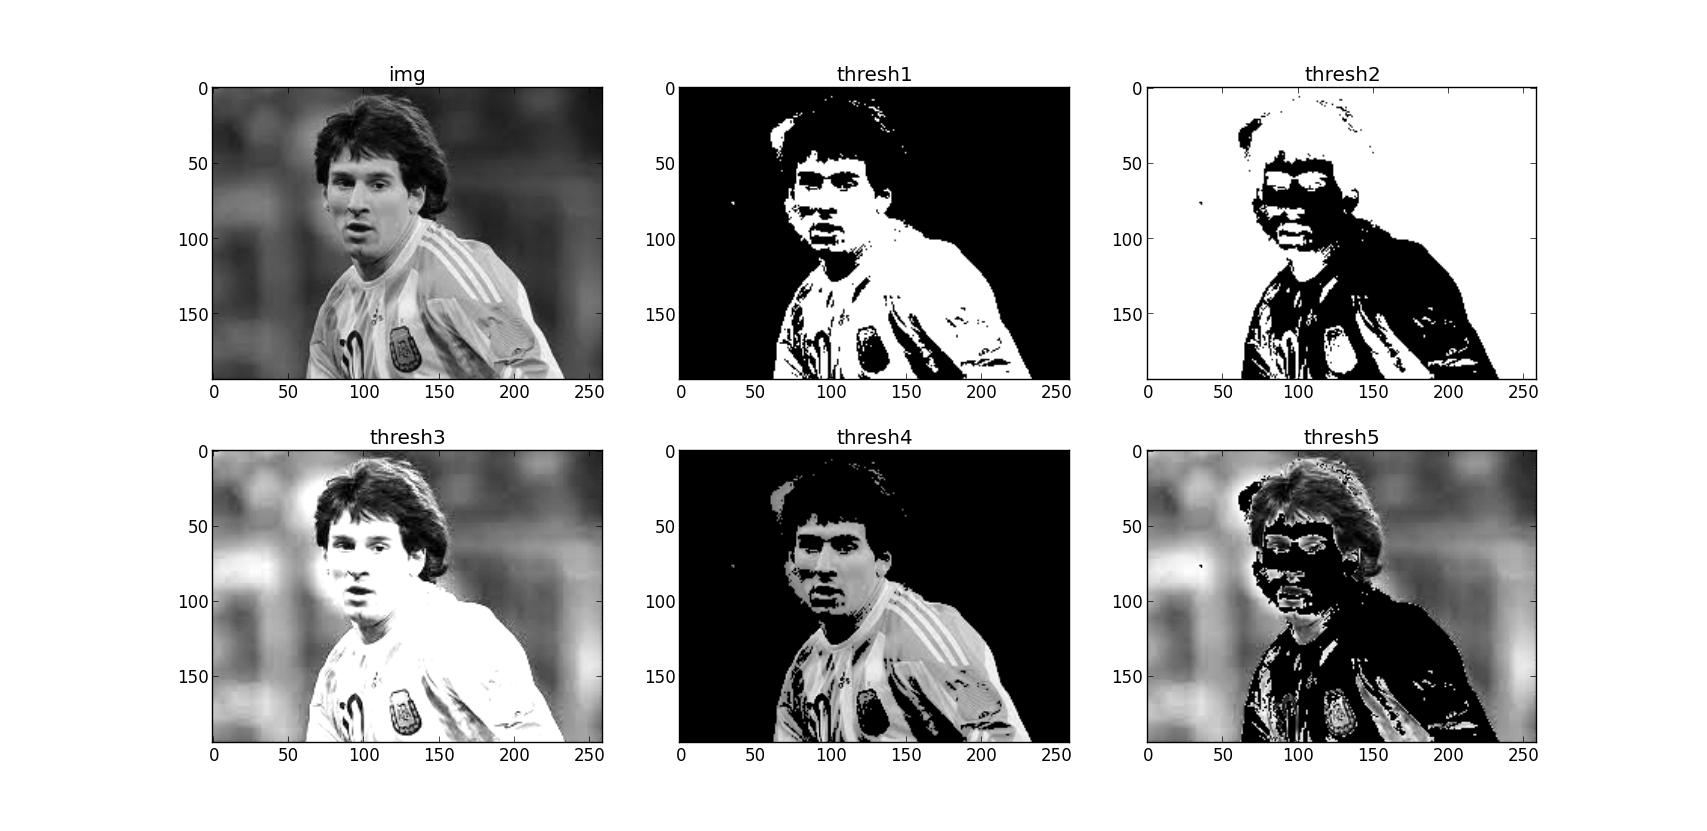
\includegraphics[scale=0.4]{img/thresh_1.png}
\caption{Simple Thresholding}
\label{fig_thresh_1}
\end{figure}

\section{Adaptive Thresholding}

In the previous section, we used a global value as threshold value. But it may not be good in all the conditions where image has different lighting conditions in different areas. In that case, we go for adaptive thresholding. In this, the algorithm calculate the threshold for a small regions of the image. So we get different thresholds for different regions of the same image and it gives us better results for images with varying illumination.\\

It has three `special' input params and only one output param.
\begin{enumerate}
	\item Adaptive Method - It decides how thresholding value is calculated.
	\begin{enumerate}
	\item cv2.ADAPTIVE\_THRESH\_MEAN\_C : threshold value is the mean of neighbourhood area.
	\item cv2.ADAPTIVE\_THRESH\_GAUSSIAN\_C : threshold value is the weighted sum of neighbourhood values where weights are a gaussian window.
    \end{enumerate}
    
    \item Block Size - It decides the size of neighbourhood area.
    \item C - It is just a constant which is subtracted from the mean or weighted mean calculated.
\end{enumerate}

Below piece of code compares global thresholding and adaptive thresholding for an image with varying illumination.

\bigskip
\begin{lstlisting}
import cv2
import numpy as np
from matplotlib import pyplot as plt

img = cv2.imread('dave.jpg',0)
img = cv2.medianBlur(img,5)

ret,th1 = cv2.threshold(img,127,255,cv2.THRESH_BINARY)
th2 = cv2.adaptiveThreshold(img,255,cv2.ADAPTIVE_THRESH_MEAN_C,\
            cv2.THRESH_BINARY,11,2)
th3 = cv2.adaptiveThreshold(img,255,cv2.ADAPTIVE_THRESH_GAUSSIAN_C,\
            cv2.THRESH_BINARY,11,2)

plt.subplot(2,2,1),plt.imshow(img,'gray')
plt.title('input image')
plt.subplot(2,2,2),plt.imshow(th1,'gray')
plt.title('Global Thresholding')
plt.subplot(2,2,3),plt.imshow(th2,'gray')
plt.title('Adaptive Mean Thresholding')
plt.subplot(2,2,4),plt.imshow(th3,'gray')
plt.title('Adaptive Gaussian Thresholding')

plt.show()
\end{lstlisting}
\bigskip

\begin{figure}[htp]
\centering
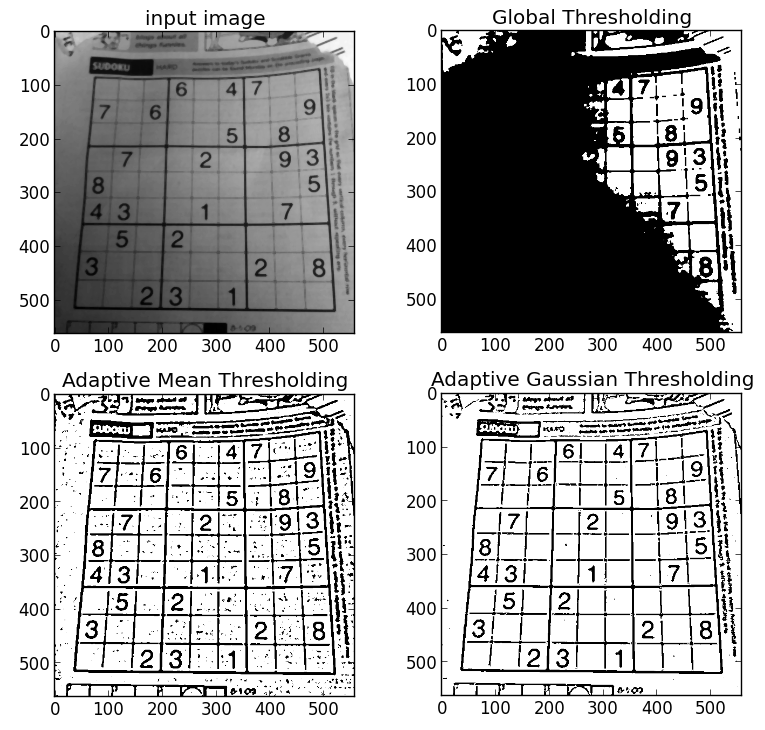
\includegraphics[scale=0.4]{img/thresh_2.png}
\caption{}
\label{}
\end{figure}

\section{Otsu's Binarization}

In the first section, I told you there is a second parameter \textbf{retVal}. Its use comes when we go for Otsu's Binarization. So what is this thing?\\

In global thresholding, we used an arbitrary value for threshold value, right? So, how can we know a value we selected is good or not? Answer is, trial and error method. But consider a bimodal image. For that image, we can approximately take a value in the middle of those peaks as threshold value, right ? That is what Otsu binarization does. \\

So in simple words, it automatically calculates a threshold value from image histogram for a \textbf{bimodal image}. \textit{(For images which are not bimodal, binarization won't be accurate.)}\\

For this, our \textbf{cv2.threshold()} function is used, but pass an extra flag, \textbf{cv2.THRESH\_OTSU}. For threshold value, simply pass zero. Then the algorithm finds the optimal threshold value and returns you as the second output, retVal. If Otsu thresholding is not used, retVal is same as the threshold value you used. \\

Check out below example. Input image is a noisy image. First I applied global thresholding for a value of 127. Then I applied Otsu's thresholding directly. Later I filtered it with a 5x5 gaussian kernel to remove the noise, then applied Otsu thresholding. See how noise filtering improves the result in Figure ~\ref{fig:thresh_3}. 

\bigskip
\begin{lstlisting}
img = cv2.imread('noisy2.png',0)

# global thresholding
ret1,th1 = cv2.threshold(img,127,255,cv2.THRESH_BINARY)

# Otsu's thresholding
ret2,th2 = cv2.threshold(img,0,255,cv2.THRESH_BINARY+cv2.THRESH_OTSU)

# Otsu's thresholding after Gaussian filtering
blur = cv2.GaussianBlur(img,(5,5),0)
ret3,th3 = cv2.threshold(blur,0,255,cv2.THRESH_BINARY+cv2.THRESH_OTSU)

# plot all the images and their histograms
titles = ['img','histogram1','th1',
          'img','histogram2','th2',
          'blur','histogram3','th3']

for i in xrange(3):
    plt.subplot(3,3,i*3+1),plt.imshow(eval(titles[i*3]),'gray')
    plt.title(titles[i*3])
    plt.subplot(3,3,i*3+2),plt.hist(eval(titles[i*3]).ravel(),256)
    plt.title(titles[i*3+1])
    plt.subplot(3,3,i*3+3),plt.imshow(eval(titles[i*3+2]),'gray')
    plt.title(titles[i*3+2])

plt.show()
\end{lstlisting}
\bigskip

\begin{figure}[htp]
\centering
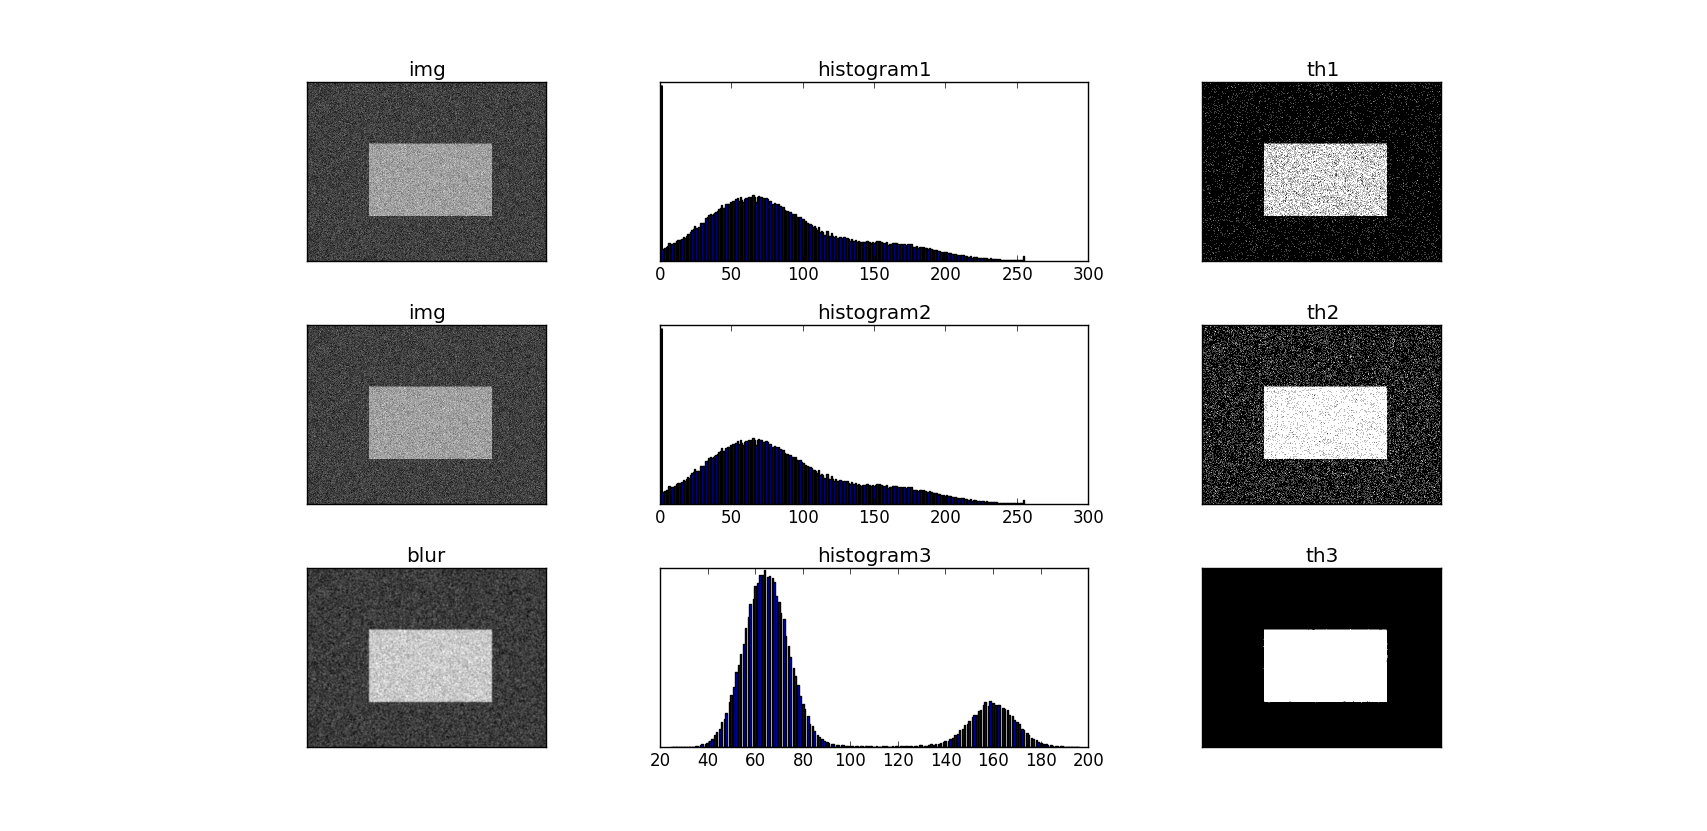
\includegraphics[scale=0.4]{img/thresh_3.png}
\caption{Otsu's Thresholding}
\label{fig:thresh_3}
\end{figure}

\subsection{How Otsu's Binarization works?}
\label{sub:Otsu_algorithm}

That is very simple. Since we are working with bimodal images, Otsu's algorithm tries to find a threshold value which minimizes the \textbf{weighted within-class variance} given by the relation :

\begin{equation} \label{eq:otsu}
 \sigma_w^2(t) = q_1(t)\sigma_1^2(t)+q_2(t)\sigma_2^2(t)
\end{equation}
where

\begin{equation}
    q_1(t) = \sum_{i=1}^{t} P(i) \quad \& \quad q_1(t) = \sum_{i=t+1}^{I} P(i) 
\end{equation}

\begin{equation}
    \mu_1(t) = \sum_{i=1}^{t} \frac{iP(i)}{q_1(t)} \quad \& \quad \mu_2(t) = \sum_{i=t+1}^{I} \frac{iP(i)}{q_2(t)}
\end{equation}

\begin{equation}
    \sigma_1^2(t) = \sum_{i=1}^{t} [i-\mu_1(t)]^2 \frac{P(i)}{q_1(t)} \quad \& \quad \sigma_2^2(t) = \sum_{i=t+1}^{I} [i-\mu_1(t)]^2 \frac{P(i)}{q_2(t)}
\end{equation}

So our plan is to find the value of \( t \) which minimizes the equation \ref{eq:otsu} and it can be done simply in Numpy as follows :

\bigskip
\begin{lstlisting}
img = cv2.imread('noisy2.png',0)
blur = cv2.GaussianBlur(img,(5,5),0)

# find normalized_histogram, and its cum_sum
hist = cv2.calcHist([blur],[0],None,[256],[0,256])
hist_norm = hist.ravel()/hist.max()
Q = hist_norm.cumsum()

bins = np.arange(256)

fn_min = np.inf
thresh = -1

for i in xrange(1,256):
    p1,p2 = np.hsplit(hist_norm,[i]) # probabilities
    q1,q2 = Q[i],Q[255]-Q[i] # cum sum of classes
    b1,b2 = np.hsplit(bins,[i]) # weights
    
    # finding means and variances
    m1,m2 = np.sum(p1*b1)/q1, np.sum(p2*b2)/q2 
    v1,v2 = np.sum(((b1-m1)**2)*p1)/q1,np.sum(((b2-m2)**2)*p2)/q2
    
    # calculates the minimization function
    fn = v1*q1 + v2*q2
    if fn < fn_min:
        fn_min = fn
        thresh = i

# find otsu's threshold value with OpenCV function 
ret, otsu = cv2.threshold(blur,0,255,cv2.THRESH_BINARY+cv2.THRESH_OTSU)
print thresh,ret
\end{lstlisting}
\bigskip

\textit{(There are some optimizations available for this algorithm and that is left for interested people.)}
\end{document}